\section{Cone square function}

In this section we show a square function estimate of the form $L^{4}(\R^{2}) \to L^{4}(\R^{3},\ell^{2})$ for solutions of the wave equation that is effectively due to \cite{MR1173929}.
\begin{lemma}[{\cite[(1.8)]{MR1173929}}]
Let $d=2$.
Let
\[
T_{\theta}f(x,t) := \chi(t) \int_{\R^{2}} K_{\theta}(x,t,y) f(y) \dif y.
\]
Then for any functions $f_{\theta,l}$ we have
\begin{equation}
\label{eq:R2-to-R3-sq-fct}
\norm[\Big]{ \Bigl( \sum_{\theta,l} \abs{T_{\theta,l}f_{\theta,l}}^{2} \Bigr)^{1/2} }_{L^{4}(\R^{3})}
\lesssim (n+1)^{5/4}
\norm[\Big]{ \Bigl( \sum_{\theta,l} \abs{f_{\theta,l}}^{2} \Bigr)^{1/2} }_{L^{4}(\R^{2})}.
\end{equation}
\end{lemma}
In \cite[(1.8)]{MR1173929} this result is stated for functions $f_{\theta,l}$ of a special form, but the proof works for arbitrary functions.
\begin{proof}
We use the classical fact that vector-valued inequalities follow from maximal inequalities.
By duality for some function $g \in L^{2}(\R^{3})$ with $\norm{g}_{2}=1$ we have
\[
LHS\eqref{eq:R2-to-R3-sq-fct}^{2}
=
\int_{\R^{3}} \sum_{\theta,l} \abs{T_{\theta,l}f_{\theta,l}}^{2} g.
\]
Since the kernels $\tilde{K}_{\theta}(x,t,\cdot) = K_{\theta}(x,t,\cdot) \chi(t)$ are uniformly integrable and by H\"older's inequality this is
\begin{align*}
&=
\int_{\R^{3}} \sum_{\theta,l} \abs[\Big]{\int_{\R^{2}} \tilde{K}_{\theta}(x,t,y) f_{\theta,l}(y) \dif y}^{2} g(x,t) \dif x \dif t\\
&\lesssim
\int_{\R^{3}} \sum_{\theta,l} \int_{\R^{2}} \abs{\tilde{K}_{\theta}(x,t,y)} \abs{f_{\theta,l}(y)}^{2} \dif y \abs{g(x,t)} \dif x \dif t\\
&=
\int_{\R^{2}} \sum_{\theta,l}  \abs{f_{\theta,l}(y)}^{2} \Bigl( \int_{\R^{3}} \abs{\tilde{K}_{\theta}(x,t,y)} \abs{g(x,t)} \dif x \dif t \Bigr) \dif y\\
&\leq
\int_{\R^{2}} \sum_{\theta,l}  \abs{f_{\theta,l}(y)}^{2} \Bigl( \sup_{\theta} \int_{\R^{3}} \abs{\tilde{K}_{\theta}(x,t,y)} \abs{g(x,t)} \dif x \dif t \Bigr) \dif y\\
&\leq
\norm[\Big]{ \sum_{\theta,l}  \abs{f_{\theta,l}(y)}^{2} }_{L^{2}_{y}(\R^{2})}
\norm[\Big]{ \sup_{\theta} \int_{\R^{3}} \abs{\tilde{K}_{\theta}(x,t,y)} \abs{g(x,t)} \dif x \dif t }_{L^{2}_{y}(\R^{2})}.
\end{align*}
Hence it remains to show the maximal inequality
\[
\norm[\Big]{ \sup_{\theta} \int_{\R^{3}} \abs{\tilde{K}_{\theta}(x,t,y)} \abs{g(x,t)} \dif x \dif t }_{L^{2}_{y}(\R^{2})}
\lesssim
(n+1)^{5/2} \norm{g}_{L^{2}(\R^{3})}.
\]
Let $\xi_{\theta}$ be a unit vector in the direction of $\theta$.
When estimating $K_{\theta}$ we have actually proved
\[
\abs{\tilde{K}_{\theta}(x,t,y)}
\lesssim_{N}
2^{3n/2} (1+2^{n} \abs{\innerp{y-x}{\xi_{\theta}}+t})^{-N} (1+2^{n/2} \abs{y-x- \innerp{y-x}{\xi_{\theta}} \xi_{\theta}})^{-N} (1+\abs{t})^{-N}.
\]
So the claimed maximal inequality will follow by scaling from a maximal inequality involving averaging over slabs of dimensions $\sim 2^{-n} \times 2^{-n/2} \times 1$ as in the picture.
\begin{center}
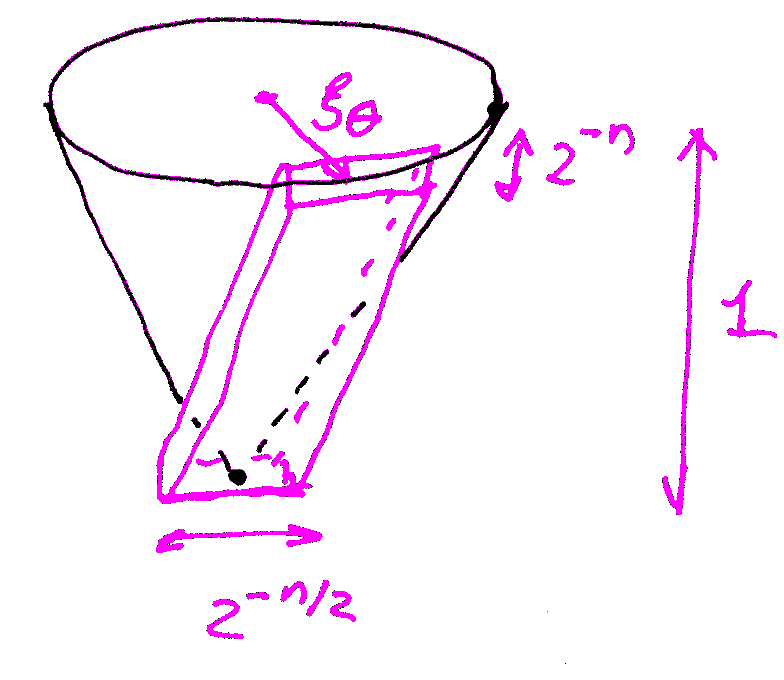
\includegraphics[height=3cm]{cone-max-fct.png}
\end{center}
We can write the average over such slab as an average over a rectangle of size $2^{-n} \times 2^{-n/2}$ in $\R^{2}$ of averages over tubes of length $1$, diameter $2^{-n}$, and slope $1$.
Hence our maximal operator is bounded by the composition of a maximal operator with $2^{n}$ separated directions in $\R^{2}$ and a maximal operator from $\R^{3}$ to $\R^{2}$ involving tubes as in Lemma~\ref{lem:R3-to-R2-tube-max-fct}.
\end{proof}
\begin{lemma}[{\cite[Lemma 1.4]{MR1173929}}]
\label{lem:R3-to-R2-tube-max-fct}
\begin{equation}
\label{eq:R3-to-R2-tube-max-fct}
\norm[\Big]{\sup_{\abs{\xi}=1} \abs[\big]{ \int_{-1}^{1} \int_{B(0,1)} g(y-\delta x-\xi t,t) \dif x \dif t} }_{L^{2}_{y}(\R^{2})}
\lesssim
(\log_{*} \delta)^{3/2}
\norm{g}_{L^{2}(\R^{3})}.
\end{equation}
\end{lemma}
Lemma~\ref{lem:R3-to-R2-tube-max-fct} extends, up to a worse exponent of $\log_{*}\delta$, (the basic version of) the maximal estimate for separated directions in $\R^{2}$ by setting $g(x,t) = g_{0}(x) \one_{[-1,1]}(t)$.
However, no proof of Lemma~\ref{lem:R3-to-R2-tube-max-fct} based on covering arguments seems to be available.
The proof uses a Sobolev embedding, $TT^{*}$, and a stationary phase decomposition.
\begin{proof}
We replace ball averages by smooth averages
\[
A_{\alpha}g(y)
:=
\int_{-1}^{1} \int_{\R^{2}} g(y-x+(\cos\alpha,\sin\alpha)t,t) \delta^{-2} \hat{a}(\delta^{-1}x) \dif x \dif t,
\]
where $\hat{a} \geq 0$ and $a$ has compact support.
Let $\tilde{g}$ denote the Fourier transform of $g$ in the $x$ variable.
Then
\[
A_{\alpha}g(y)
=
\int_{-1}^{1} \int_{\R^{2}} e(\innerp{y+(\cos\alpha,\sin\alpha)t}{\xi}) \tilde{g}(\xi,t) a(\delta \xi) \dif \xi \dif t.
\]
We decompose $a(\delta\cdot) = a_{0} + \sum_{\lambda}a_{\lambda}$, where $a_{0}$ is a bump function supported on the unit ball and each $a_{\lambda}$ is a bump function supported on on a dyadic annulus of radius $\sim\lambda$, so that there are $\sim \log_{*}\delta$ different $\lambda$'s.
The contribution of $a_{0}$ can be easily estimated by going back to the spatial formulation.

Hence it suffices to show that for
\[
A_{\alpha}^{\lambda} g(y)
:=
\int_{-1}^{1} \int_{\R^{2}} e(\innerp{y+(\cos\alpha,\sin\alpha)t}{\xi}) \tilde{g}(\xi,t) a_{\lambda}(\xi) \dif \xi \dif t
\]
we have the estimates
\[
\norm{ \sup_{\alpha} \abs{A_{\alpha}^{\lambda} g}}_{L^{2}(\R^{2})}
\lesssim
(\log_{*} \lambda)
\norm{ g }_{L^{2}(\R^{3})}.
\]
Indeed, summing these estimates we would obtain
\[
\sum_{\lambda} (\log_{*} \lambda) \norm{ P_{\lambda} g }_{L^{2}(\R^{3})}
\lesssim
(\log_{*} \delta)^{3/2} \bigl( \sum_{\lambda} \norm{ P_{\lambda} g }_{L^{2}(\R^{3})}^{2} \bigr)^{1/2}
\lesssim
(\log_{*} \delta)^{3/2} \norm{ P_{\lambda} g }_{L^{2}(\R^{3})}
\]
where $P_{\lambda}$ is the Fourier projection to the support of $a_{\lambda}$.
In order to show the claim we decompose further
\[
a_{\lambda} = a_{\lambda,0} + \sum_{0<k\lesssim \log_{*}\lambda} a_{\lambda,k},
\]
where
\[
a_{\lambda,k}(\xi,\alpha) = a_{\lambda}(\xi) \beta(2^{-k}\lambda^{1/2}\innerp{(-\sin\alpha,\cos\alpha)}{\frac{\xi}{\abs{\xi}}})
\]
and $\beta$ is a smooth function supported on $\pm [1/2,2]$ such that $\sum_{k\in\Z} \beta(2^{-k}s)=0$ for $s\neq 0$.
Let
\[
A_{\alpha}^{\lambda,k} g(y)
:=
\int_{-1}^{1} \int_{\R^{2}} e(\innerp{y+(\cos\alpha,\sin\alpha)t}{\xi}) \tilde{g}(\xi,t) a_{\lambda,k}(\xi,\alpha) \dif \xi \dif t.
\]
It suffices to show
\[
\norm{ \sup_{\alpha} \abs{A_{\alpha}^{\lambda,k} g}}_{L^{2}(\R^{2})}
\lesssim
\norm{ g }_{L^{2}(\R^{3})}.
\]
An estimate for fixed $\alpha$ is relatively easy.
To proceed we use the inequality
\begin{multline*}
\sup_{\alpha \in [0,2\pi]} \abs[\big]{F(\alpha)^{2} - F(0)^{2}}
=
\sup_{\alpha \in [0,2\pi]} \abs[\Big]{ 2 \int_{\alpha'=0}^{\alpha} F(\alpha') F'(\alpha') \dif \alpha'}\\
\leq
2 \int_{\alpha=0}^{2\pi} \abs{F(\alpha)} \abs{F'(\alpha)} \dif \alpha
\leq
2 \Bigl( \int_{\alpha=0}^{2\pi} \abs{F(\alpha)}^{2} \dif \alpha \Bigr)^{1/2}
\Bigl( \int_{\alpha=0}^{2\pi} \abs{F'(\alpha)}^{2} \dif \alpha \Bigr)^{1/2}.
\end{multline*}
Applying this inequality with $F(\alpha)=A_{\alpha}^{\lambda,k}g(y)$ we see that it suffices to show
\begin{equation}
\label{eq:MSS92-sq-fct-after-Sobolev-emb}
\Bigl( \int_{\R^{2}} \int_{\alpha=0}^{2\pi} \abs{A_{\alpha}^{\lambda,k} g(y)}^{2} \dif \alpha \dif y \Bigr)
\Bigl( \int_{\R^{2}} \int_{\alpha=0}^{2\pi} \abs{\partial_{\alpha} A_{\alpha}^{\lambda,k} g(y)}^{2} \dif \alpha \dif y \Bigr)
\lesssim
\norm{ g }_{L^{2}(\R^{3})}^{4}.
\end{equation}
Consider the first bracket.
Expanding the square we obtain
\begin{multline*}
\int_{\R^{2}} \int_{\alpha=0}^{2\pi} \int e(\innerp{y+(\cos\alpha,\sin\alpha)t}{\xi}-\innerp{y+(\cos\alpha,\sin\alpha)t'}{\xi'}) \\
\cdot \tilde{g}(\xi,t) a_{\lambda,k}(\xi,\alpha) \overline{\tilde{g}(\xi',t') a_{\lambda,k}(\xi',\alpha)} \dif \xi \dif \xi' \dif t \dif t' \dif \alpha \dif y\\
=
\int e(\innerp{y+(\cos\alpha,\sin\alpha)t}{\xi}) \\
\cdot \tilde{g}(\xi,t) a_{\lambda,k}(\xi,\alpha) \FT(\overline{\tilde{g}(\cdot,t') a_{\lambda,k}(\cdot,\alpha)})(y+(\cos\alpha,\sin\alpha)t') \dif \xi \dif t \dif t' \dif \alpha \dif y\\
=
\int e((t-t')\innerp{(\cos\alpha,\sin\alpha)}{\xi}) \\
\cdot \tilde{g}(\xi,t) a_{\lambda,k}(\xi,\alpha) \overline{\tilde{g}(\xi,t') a_{\lambda,k}(\delta \xi)} \dif \xi \dif t \dif t' \dif \alpha\\
=
\int H^{\lambda,k}(t,t',\xi) \tilde{g}(\xi,t) \overline{\tilde{g}(\xi,t')} \dif \xi \dif t \dif t',
\end{multline*}
where
\[
H^{\lambda,k}(t,t',\xi)
=
\int_{\alpha=0}^{2\pi} e((t-t')\innerp{(\cos\alpha,\sin\alpha)}{\xi}) \abs{a_{\lambda,k}(\xi,\alpha)}^{2} \dif \alpha.
\]
We claim that this function satisfies
\begin{equation}
\label{eq:MSS92-TT*}
\abs{H^{\lambda,k}(t,t,\xi)}
\lesssim_{N}
\lambda^{-1/2}2^{k} (1+2^{2k}\abs{t-t'})^{-N},
\quad
\abs{\xi}\sim\lambda,\,
\abs{t}\leq 1,\,
\abs{t'}\leq 1.
\end{equation}
For $k>0$ this is an oscillatory integral estimate.
Indeed, $a_{\lambda,k}(\xi,\cdot)$ is supported on a set of measure $\sim 2^{k} \lambda^{-1/2}$ and its $m$-th derivative is bounded by $(2^{-k}\lambda^{1/2})^{m}$.
So after the change of variable $\alpha= \alpha' 2^{k}\lambda^{-1/2}$ the amplitude becomes a smooth function with uniform bounds on the support and all derivatives.
The phase becomes
\[
(t-t') \abs{\xi} \innerp{(\cos(2^{k}\lambda^{-1/2}\alpha'),\sin (2^{k}\lambda^{-1/2}\alpha'))}{\frac{\xi}{\abs{\xi}}}.
\]
By construction the first derivative of the phase is
\begin{multline*}
(t-t') \abs{\xi} 2^{k}\lambda^{-1/2} \innerp{(-\sin(2^{k}\lambda^{-1/2}\alpha'),\cos (2^{k}\lambda^{-1/2}\alpha'))}{\frac{\xi}{\abs{\xi}}}\\
\sim
(t-t') \abs{\xi} 2^{k}\lambda^{-1/2} (2^{k}\lambda^{-1/2})
\sim
2^{2k} (t-t')
\end{multline*}
on the support of the phase.
On the other hand, for $m\geq 2$ the $m$-th derivative of the phase is bounded by
\[
(t-t') \abs{\xi} (2^{k}\lambda^{-1/2})^{m}
\lesssim
(t-t') \abs{\xi} (2^{k}\lambda^{-1/2})^{2}
=
2^{2k} (t-t').
\]
Hence \eqref{eq:MSS92-TT*} follows by partial integration.
Using \eqref{eq:MSS92-TT*} we obtain
\begin{multline*}
\int \abs{H^{\lambda,k}(t,t',\xi)} \abs{\tilde{g}(\xi,t) \tilde{g}(\xi,t')} \dif \xi \dif t \dif t'\\
\lesssim_{N}
\lambda^{-1/2}2^{k} \int (1+2^{2k}\abs{t-t'})^{N} \abs{\tilde{g}(\xi,t) \tilde{g}(\xi,t')} \dif \xi \dif t \dif t'\\
\lesssim
\lambda^{-1/2}2^{k} 2^{-2k} \norm{g}_{2}^{2}
=
\lambda^{-1/2}2^{-k} \norm{g}_{2}^{2}
\end{multline*}
provided that $N>1$.
The estimate for the term involving $\partial_{\alpha}$ is similar with the following changes: when in
\[
\partial_{\alpha} \Bigl( e(\innerp{y+(\cos\alpha,\sin\alpha)t}{\xi}) a_{\lambda,k}(\xi,\alpha) \Bigr)
\]
the derivative falls on $a_{\lambda,k}$ we lose an additional factor $2^{-k}\lambda^{1/2}$.
If on the other hand the derivative falls on the exponential we get
\[
t \abs{\xi} 2^{k} \lambda^{-1/2} e(\innerp{y+(\cos\alpha,\sin\alpha)t}{\xi})
\underbrace{2^{-k}\lambda^{1/2 }\innerp{(-\sin\alpha,\cos\alpha)}{\frac{\xi}{\abs{\xi}}}}
a_{\lambda,k}(\xi,\alpha).
\]
The underlined function can be absorbed in $a_{\lambda,k}$ by changing the function $\beta$, and we lose a factor $t \abs{\xi} 2^{k} \lambda^{-1/2} \lesssim 2^{k} \lambda^{1/2}$.
Since there are two derivatives $\partial_{\alpha}$ we actually lose $(2^{k}\lambda^{1/2})^{2}$, and we obtain
\[
\int_{\R^{2}} \int_{\alpha=0}^{2\pi} \abs{\partial_{\alpha} A_{\alpha}^{\lambda,k} g(y)}^{2} \dif \alpha \dif y
\lesssim
\lambda^{-1/2}2^{-k} (2^{k}\lambda^{1/2})^{2} \norm{g}_{2}^{2}.
\]
Multiplying this with the previous estimate gives \eqref{eq:MSS92-sq-fct-after-Sobolev-emb} for $k>0$.

Finally, the $k=0$ case of the estimate \eqref{eq:MSS92-TT*} is even easier because we do not claim any decay in $\abs{t-t'}$, so no partial integration is needed.
\end{proof}

%%% Local Variables:
%%% mode: latex
%%% TeX-master: decoupling-notes
%%% End:
